\section{Wave Equation}
\label{sec:wave}
%From the wave kernel form, to the wave equation as your wish
%With the HLE Vlasov solver for the particle dynamics, 
We now couple the HLE Vlasov solver with the wave equation to self-consistently study the resonant wave-particle interactions. 
%In our theoretic framework, We write 
%We here show the derivation of the equation with resepct to the slowly varying wave envelope from the above definition.
%From the Maxwell equation, we can derive the equation regarding the envelope as
%\begin{equation}\label{eq.wavegen}
%\begin{aligned}
%    &-\nabla^2 \mathbf{a}+ \frac{\partial^2 \mathbf{a}}{\partial t^2}
%    \\
%    &+ (2 \imath \omega) \frac{\partial \mathbf{a}}{\partial t}-2 \imath(\mathbf{k} \cdot \nabla) \mathbf{a}+\imath(\nabla \cdot \mathbf{a}) \mathbf{k}+\imath \nabla \mathbf{a} \cdot \mathbf{k}
%    \\
%    &= 4 \pi \left(\mathbf{j}_c+\mathbf{j}_p\right)
%    \end{aligned}
%\end{equation}
%where $\mathbf{j}_c$ is the envelope of the background plasma current, and $\mathbf{j}_p$ is the current from perturbed distribution. The fast varying phase $\phi_f$ has been substracted from the wave equation.
%
%If one consider the slowying varying envelope approximation \cite{svap}, or equivalently, the narrow-banded approximation, the higher order derivative terms of the amplitude can be neglected, and leaves a advective type wave equation
%\begin{equation}
%    \frac{\partial \mathbf{a}}{\partial t} + \mathbf{v}_g \cdot \frac{\partial \mathbf{a}}{\partial s} = \left[\frac{\partial \mathcal{D}}{\partial \omega}\right] \cdot \mathbf{j}_p~.
%\end{equation}
%
%benchmark one chorus wave
%equations for the wave 
Here we consider the interaction between energetic electrons and  chorus waves in the magnetosphere.
The  chorus is a circularly polarized electromagnetic wave
propagating along the Earth's dipole magnetic field. 
The vector potential $\mathbf{A}(s,t)$ for the transverse wave is written as
\begin{equation}
    \mathbf{A}(s,t) = \mathbf{a}(s,t)e^{\imath \phi_f},.
\end{equation}
where $\phi_f$ is the fast varying phase and $\mathbf{a}(s,t)$ is the slowly varying envelope of the wave packet. 
The second order wave equation for the chorus in the resonant frame  is 
\begin{equation}\label{eq.Wave}
    \begin{aligned}
        &\frac{\partial^2 a}{\partial t^2} - \frac{\partial^2 a}{\partial s_i^2} + {2\imath\omega_l}\frac{\partial a}{\partial t} + 2\imath k_l\frac{\partial a}{\partial s_i} + \\
        &\frac{\omega_p^2 \omega_{ce}}{(\omega_{ce}-\omega_l)} \int_0^t d \tau \frac{\partial a}{\partial \tau} e^{-\imath\left(\omega_l-\omega_{c e}\right)(t-\tau)} = {4\pi}j_p~,
        \end{aligned}
      \end{equation}
where 
%the  vector potential has been  represented by complex number, 
$a = a_x + \imath a_y$ with $x$ and $y$ the directions 
%basis vector 
perpendicular to the  magnetic field. The plasma current consists of the currents from cold electrons and energetic electrons and the cold electron current can be analytically integrated.
We write the second-order wave equation (\ref{eq.Wave}) in the normalized form as
\begin{equation}\label{eq.Wave2}
    \begin{aligned}
        \frac{d y_0}{d t} & =y_1 
        \\
        \frac{d y_1}{d t} & =-2 \imath \omega_l y_1+\frac{\partial^2 y_0}{\partial s^2}-2 \imath k_l \frac{\partial y_0}{\partial s}- \frac{\omega^2_p\omega_{ce}}{\omega_{ce}-\omega_l}y_{2} +j_p\\
        \frac{d y_2}{d t} & =y_1-\imath\left(\omega_l-\omega_{ce}\right) y_2~,
        \end{aligned}
\end{equation}
where 
%the followying terms and integral form are used to simplify the equation
\begin{equation}
    \begin{aligned}
        y_0 &= a(s_i,t)~,
        \\
        y_1 &= \frac{\partial a(s_i,t)}{\partial t}~,
        \\
        y_2 &= e^{-\imath(\omega_l-\omega_{ce})t} \int_0^t\mathrm{d}\tau \frac{\partial a}{\partial \tau} e^{\imath(\omega_l-\omega_{ce})\tau}~.
    \end{aligned}
\end{equation}
The first and second order spatial derivatives are given by central difference scheme
\begin{equation}
    \begin{aligned}
    f'(x) &\approx \frac{f(x + h) - f(x - h)}{2h}\\
    f''(x) &\approx \frac{f(x + h) - 2f(x) + f(x - h)}{h^2}
    \end{aligned}
\end{equation}
The energetic electron
current $j_p$ is obtained from the perpendicular velocity moment of energetic particle distribution,
\begin{equation}
    j_p(s_i,t) = - \frac{n_{h0}k_l(t)}{4\pi}\iiint \sqrt{2m_e\omega_{ce}(s)(\mathcal{J}+\Omega+\Pi_i)}f e^{\imath \xi} \rm d \xi \rm d \Omega \rm d \mathcal{J}~,
\end{equation}
where $n_{h0}$ is the density ratio of the energetic electrons to the background cold plasmas.
The current integral is solved by interpolating method order by order.
%The term on the right side are all determined and the rest of the Equations (\ref{eq.Wave}) are 
The coupled ODEs (\ref{eq.Wave2}) with respect to time  
are then solved by the RK method. 



%We can further neglect
 To check the contribution of the second order derivatives of slowly varying kernel $a(s_i,t)$ in the wave equation (\ref{eq.Wave}), 
 we further simplify the integral term and obtain the first-order advective wave equation 
\begin{equation}\label{eq.Wave1st}
    \frac{\partial a}{\partial t} + v^l_{g} \frac{\partial a}{\partial s_i} = \frac{2\pi v^l_g}{k_l} j_{p}~,
\end{equation}
where $v_g^l$ is the linear group velocity.
%  and for the whistler chorus, it is 
% \begin{equation}
%     v_g^l = \frac{2k_l}{2\omega_l + \omega_p^2 \omega_{ce}/(\omega_{ce}-\omega_l)^2}
% \end{equation}
% The approximation is equivlent to the WKB approximation which is valid for most cases of the chorus wave evolution, and can greatly reduce the numerical workload.In the meantime, 
For the first-order advective wave equation (\ref{eq.Wave1st}), we apply a simple implicit upwind scheme to solve such equation,
\begin{equation}
    %a^{n+1}_k = a^{n}_k \pm {u_k} (a_{k\pm1}^{n+1} - a_{k}^{n+1})\frac{\Delta t}{\Delta s}
    \begin{aligned}
    a^{n+1}_k &= \left[ S_k^n \pm  \frac{\mathrm{imp}}{\Delta s}  {u_k} a_{k\pm1}^{n+1} + \left(\frac{1}{\Delta t} - \frac{(1- \mathrm{imp})}{\Delta s} u_k\right)  a_{k}^{n} \pm  \frac{(1-\mathrm{imp})}{\Delta s} u_k a_{k \pm 1}^{n} \right]/\left(\frac{1}{\Delta s} + \frac{\mathrm{imp}}{\Delta s}u_k\right)
    \end{aligned}
\end{equation}
where $u_k = v_g(s=s_k)$, $S_k$ is the source term in the right-hand-side of Eq. (\ref{eq.Wave1st}), $\mathrm{imp}$ is the combination factor of the implicit-explicit upwind scheme. 
%a constant from 0 to 1, denotes fully explicit and fully implicit. 
The sign of the advective term depends on the direction of the group velocity. The absorption boundary condition and fixed noisy initialization condition are applied at the ends of the domain.

%Here, we examine the wave equation order effect in
As shown in Fig.~\ref{fig.cmp2}, 
%the differences of the wave amplitudes from 
the first-order wave equation show good approximation to the second-order wave equation and  
%The results show a tiny difference, 
thus 
 the second order term in Eq. (\ref{eq.Wave})
may be neglected for the simulation of the onset of chorus wave frequency chirping
for computation efficiency.

%is valid.At most of the simulation periods, the results are in good accordence until the frequency is modified too much. At such stage, the onset approximation is no longer valid. Therefore, we apply the first-order for efficient which is valid during the onset stage.

\begin{figure}[htbp]
    \centering
    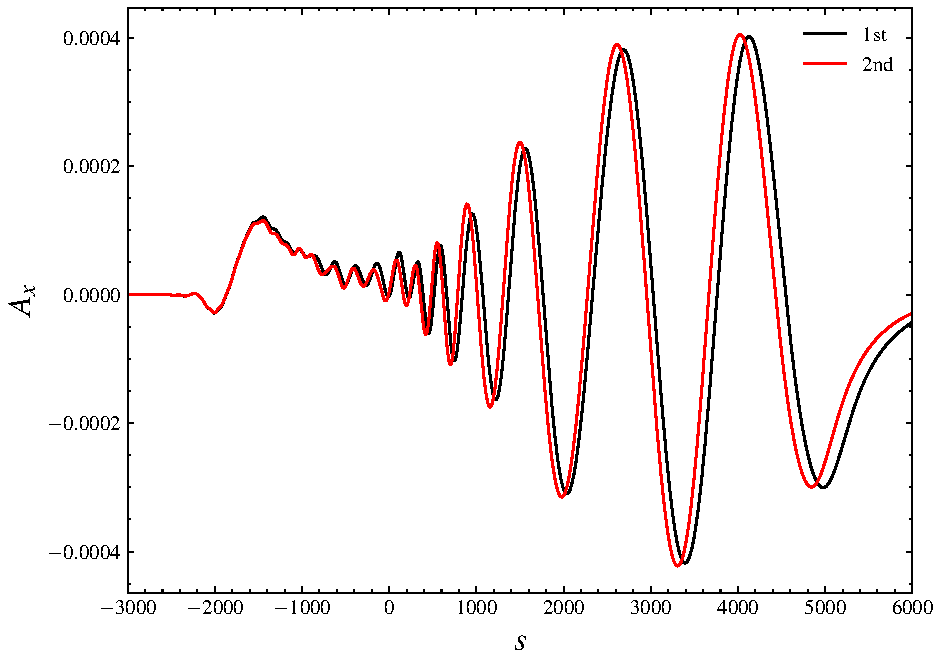
\includegraphics[scale=0.5]{cpc_img/fig_diff.pdf}
    \caption{
Wave amplitudes calculated 
    %The difference of the wave snapshot 
    from the second-order and first-order wave equations. 
    }
    \label{fig.cmp2}
\end{figure}